\section{Localisation}
Mobile robots, navigating in accordance to a map, need localisation.
There a various localisation methods and sensors for mobil robots.
This section describes how a localisation method was implemented on a ''Nexus Robot''
with data from the robot's encoders and it's laserrange scanner.
\subsection{Method}
For the localisation part of the project it was chosen to compare two different approaches:

\begin{itemize}
	\item Position estimate based on odometry (wheel encoders).
	\item Position estimate based on line features extracted from the laserrange scanner. 
\end{itemize}

Both of these approaches rely on a known starting location. The second also needs knowledge of the environment - it must  compare the extracted features with probable features from the map (based on last know location of the robot). 


The mobile robot used is a "Nexus Robot - 2WD mobile robot kit 10004", fitted with a laserrange scanner of type "Hokuyo URG-04LX-LG". 

\begin{figure}[ht]
\centering
  \begin{subfigure}[t]{0.3\textwidth}
    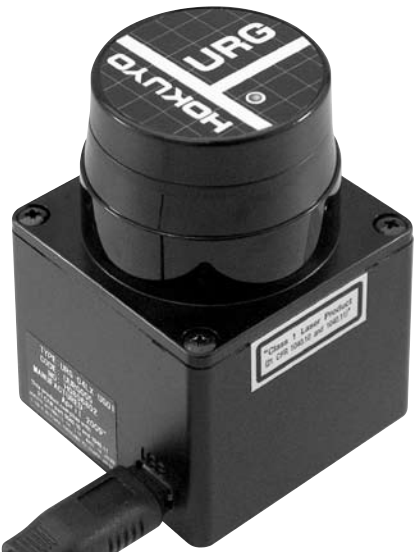
\includegraphics[width = \textwidth]{graphics/hokuyo_laserrange}
    \caption{Hokuyo URG-04LX-LG laserrange scanner.}
    \label{laserrange}
  \end{subfigure}
  \begin{subfigure}[t]{0.4\textwidth}
    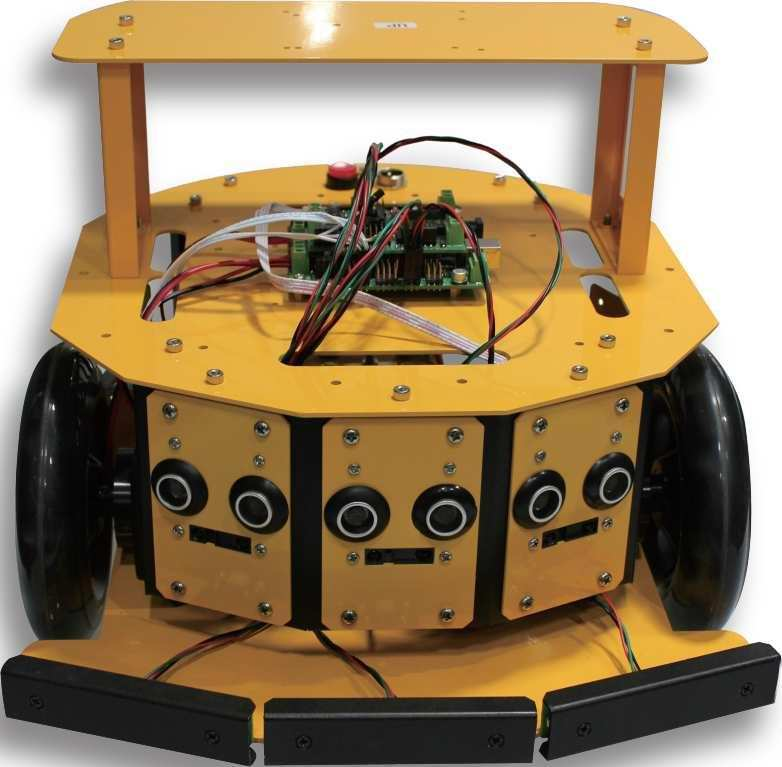
\includegraphics[width = \textwidth]{graphics/nexus_robot}
    \caption{Nexus Robot - 2WD mobile robot kit 10004}
    \label{laserrange}
  \end{subfigure}
\end{figure}

\subsubsection{Gathering data using UMB-mark}
The performance of the localization technique was measured using UMB-mark. 
The position before and after following a preprogrammed path through a 1 x 1 [m] square 5 times was compared. The planned path is shown in figure \todo[inline, author=Michael]{I need picture of it here..}
While testing, the robot was not given any feedback from the sensors. After each $90 \deg$ turn, the robot stopped and its position on the test track was measured for reference.  
Sensor readings from both the encoders and the laserrange scanner was gathered, and saved for further offline processing. 
This means that 3 different measurements of the position was gathered: 
\begin{itemize}
	\item Reference position (measured with tape)
	\item Position based on encoder feedback. 
	\item Position based on feature extraction using the laser range scanner. 
\end{itemize}

\subsubsection{Position based on odometry}
\todo[inline, author=Michael]{Based on (or ripped off :P ) sec. 5.2.4 from our lovely friend, siegwart.}
The position/state of the robot is represented by the vector: 
\begin{equation}
  Q = 
  \begin{bmatrix}
    x \\
    y \\
    \alpha
  \end{bmatrix}
\end{equation}
The robots position is estimated from the previous position + the movement in the last time period $\Delta t$. The change in position $\Delta Q$ from each timestep is added to the position. This can be written as 
\begin{equation}
  Q\textrm' = Q + \Delta Q
\end{equation}
The feedback from the robot is given as the movement of each wheel in millimetres. $\Delta Q$ can be found from the following equations: 
\begin{eqnarray}
	\Delta x &=& \Delta s \cos \left(\alpha + \frac{\Delta \alpha}{2}\right) \\
	\Delta y &=& \Delta s \sin \left(\alpha + \frac{\Delta \alpha}{2}\right) \\
	\Delta \alpha &=& \frac{\Delta s_r + \Delta s_l}{b} \\
	\Delta s &=& \frac{\Delta s_r + \Delta s_l}{2} \\
\end{eqnarray}
Where $\Delta s_r; \Delta s_l$ = distance traveled by right and left wheel and $b$ is the distance between the robots two wheels. Adding this together, the equation for the updated position is: 
\begin{equation}
  Q\textrm' = 
  \begin{bmatrix}
    x \\
    y \\
    \alpha
  \end{bmatrix}
  +
  \begin{bmatrix}
    \Delta s \cos \left(\alpha + \frac{\Delta \alpha}{2}\right) \\
    \Delta s \sin \left(\alpha + \frac{\Delta \alpha}{2}\right) \\
    \frac{\Delta s_r + \Delta s_l}{b}
  \end{bmatrix}
\end{equation}
\todo[inline, author=Michael]{Maybe add an interfacing of scanner subsubsection here?}
\todo[inline, author=Michael]{And so he wrote a section :P}
\subsubsection{Getting data from the laser range scanner}
The Hokuyo laser scanner measures distance to the nearest obstacles in a $240 \degree$ range. The angular resolution is $0.352 \degree$ which gives 681 data points for each scan. The scanning rate is 10 Hz.

The laser range scanner communicates with the computer using Serial over USB. The serial communication uses the SCIP 2.0 serial protocol. 
A basic application for gathering data from the laser range was written in C++.\footnote{The program is called "hokuyo\_laserrange" in the included "Code" directory} 
The program gathers and decodes the data received, and saves it as a CSV file. The program stops the laser range scanner whenever the UMBmark test is terminated.

\input{./content/localisation/ransac}

\subsubsection{Position based on features from laserrange scanner}

\begin{figure}
  \includestandalone{./content/localisation/flowchart}
  \caption{The localisation method}
  \label{fig:localisation}
\end{figure}

